\section{Experiments}
\label{sec:experiments}
We evaluate the MGPA construction in three steps: controlled measurements
test selective correction and its components; recorded EEG tests source
attenuation alongside task utility; cross-task reuse tests whether one
selected correction can improve other frozen predictors. Closed-form and
Iterative MGPA share the same principle and pooled conditional target.
Their comparison examines complementary constructions, while targeted
ablations isolate the gate, target and nonlinear critic.

\subsection{Experimental design and evaluation}
\label{sec:protocol}
\paragraph{Evaluation.}
Source accessibility and downstream utility answer different questions:
information readable by a source probe need not be used by a task head.
We report source AUROC $S$ from the strongest independent reader in a
declared bank, and task AUROCs for heads trained before correction
($T_f$, frozen) or after correction ($T_r$, refitted).
These distinguish compatibility with an existing predictor from utility
after head retraining. Task scores average the two cross-source transfer
directions; recorded SSVEP uses twelve-class macro AUROC.
Movement $M$ is the participant-mean relative embedding displacement.
The reuse study instead evaluates fixed heads across device--label
associations and a separate control head trained without that association.

\paragraph{Fitting and comparison.}
Participant roles separate adapter fitting, validation, reader training
and evaluation. MGPA fitting uses source labels and calibration
contrasts, not downstream labels. Controlled gate comparisons and the
supplementary N170 comparison with IGBP match validation movement budgets;
main recorded comparisons use native outputs. Reuse selects an operating point on
P300 development data, then holds it fixed on all evaluation tasks.
Identity, LEACE and IGBP are source-blind comparators. CORAL and paired affine
FEATMAP use source identity at application and are grouped separately.
Iterative results average three fitted trajectories. Key contrasts use
paired 95\% participant-bootstrap intervals. Appendix~\ref{app:protocols}
gives the splits, fitting repetitions, comparator settings, reader banks
and uncertainty calculation.

\subsection{Controlled tests of the MGPA construction}
\label{sec:gate-result}
\paragraph{Selective correction from paired measurements.}
Using wet trials from the 102-participant SSVEP collection \citep{zhu2021ssvep}, we
encode each trial under common-average and Oz references. Full reference
contrasts provide calibration; evaluated views use a scaled embedding
contrast ($\gamma=.005$). Source assignment is associated with stimulus
frequency during adapter fitting and balanced during evaluation.
The source--task association makes source prediction an ambiguous guide to
correction. Same-trial calibration supplies measurement evidence; the
experiment tests whether MGPA can use it to attenuate source information
while retaining the correlated task signal.

\begin{table}[htbp]
\centering\small
\caption{\textbf{Selective correction with a single analytic map.}
Controlled SSVEP at native endpoints: independent source AUROC,
frozen/refitted task AUROC and relative movement. All methods share a reader
realization over four rotations (81 distinct evaluation participants).
Source-aware rows require source identity.
Paired contrasts are in Appendix~\ref{app:closed-form-controlled}.}
\label{tab:controlled-cf}
% Generated by build_experiment_assets.py; see experiment_provenance.json.
\begingroup\small\setlength{\tabcolsep}{4pt}
\begin{tabular}{@{}llrrrr@{}}
\toprule
Interface & Method & Source $\downarrow$ & Frozen $\uparrow$ & Refitted $\uparrow$ & Movement \\
\midrule
\multirow{3}{*}{\shortstack[l]{\emph{Source-blind}\\\emph{correction}}} & Identity & 0.683 & 0.753 & 0.753 & 0.000 \\
 & LEACE & 0.660 & 0.656 & 0.665 & 0.120 \\
 & \textbf{MGPA-CF} & 0.510 & 0.753 & 0.753 & 0.028 \\
\midrule
\multirow{4}{*}{\shortstack[l]{\emph{Source-aware}\\\emph{alignment}}} & CORAL $\to$ ref. 0 & 0.502 & 0.753 & 0.753 & 0.012 \\
 & CORAL $\to$ ref. 1 & 0.502 & 0.753 & 0.753 & 0.012 \\
 & FEATMAP $\to$ ref. 0 & 0.502 & 0.753 & 0.753 & 0.012 \\
 & FEATMAP $\to$ ref. 1 & 0.502 & 0.753 & 0.753 & 0.012 \\
\bottomrule
\end{tabular}\endgroup

\end{table}

Closed-form MGPA brings source accessibility near chance while retaining
frozen-task performance (Table~\ref{tab:controlled-cf}). Relative to LEACE,
the paired source
change is $-.1496$ $[-.1580,-.1426]$ and the frozen-task gain is $.0964$
$[.0831,.1097]$.
Routed CORAL and FEATMAP also attain near-chance source
scores and retain task quality, using the known measurement condition.

\paragraph{Constraining critic-driven corrections.}
Do critic-driven updates benefit from measurement-derived rather than
generic edit permissions? We compare measurement, same-rank PCA/random
and ungated updates, holding the critic bank, solver, stage budget and
original-$Q_0$ anchor input fixed; only measurement-gated edits preserve
$Q_0$. A separate target comparison holds the gate and remaining procedure
fixed, contrasting conditional and empirical unconditional mean-score anchoring.

\begin{figure}[htbp]
\centering
% Original bar-panel version remains in controlled_mechanisms.pdf.
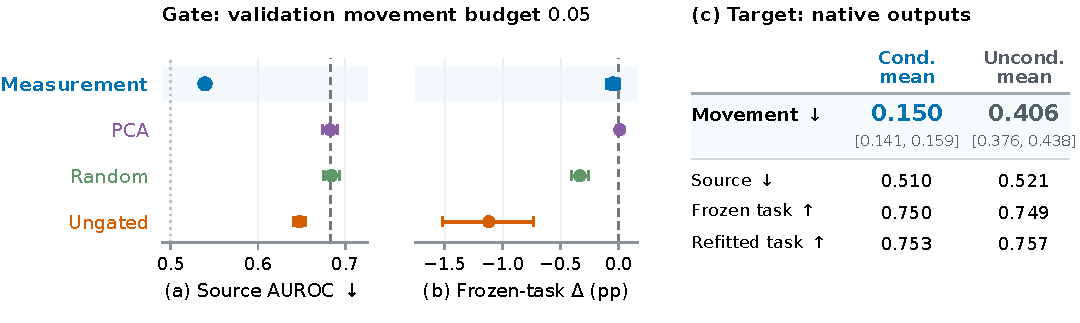
\includegraphics[width=\linewidth]{assets/controlled_mechanisms_compact.pdf}
\caption{\textbf{Where correction acts and what it targets.}
\emph{(a--b) Gate:} source AUROC and paired frozen-task change from identity at a common
$.05$ validation movement budget; dashed lines mark identity and the dotted
line marks chance. Random averages five orientations.
\emph{(c) Target:} conditional versus empirical unconditional mean-score
anchoring, with native 48-stage movement and source/task AUROC.
Three fits, 81 participants; whiskers and movement brackets give 95\%
participant-bootstrap intervals. Budget-matched gates and native target endpoints are separate comparisons.}
\label{fig:gate}
\label{fig:target-cost}
\end{figure}

Measurement-gated correction suppresses source more strongly than all
three controls (Figure~\ref{fig:gate}a). Its frozen-task change from identity is
$-.0005$ $[-.0010,.0001]$, and its advantage over ungated correction is
$.0107$ $[.0069,.0147]$. Attained evaluation movements span $.0504$--$.0539$.
The result distinguishes measurement-supported directions from a generic
restriction of rank or movement. Appendix~\ref{app:gate-attribution}
details the comparison.

\paragraph{Conditioning reduces correction cost.}
\label{sec:ablations}
Conditional-mean anchoring uses $M=.1500$ rather than $.4063$ for the
empirical unconditional mean-score target, which requires about 2.7 times
as much movement (Figure~\ref{fig:target-cost}c). Source AUROC is lower
($.5105$ versus $.5214$), with no clear frozen-task difference; refitted-task
AUROC favors the unconditional target ($.7574$ versus $.7527$).
This links the cost argument in Section~\ref{sec:targets} to learned
correction. Unlike the fixed-score analysis, these trajectories refit their
critics separately. Appendix~\ref{app:target-controls} gives the target
definitions and paired contrasts.

\subsection{Correction on recorded EEG}
\label{sec:real-results}
We next test the construction on two forms of recorded EEG:
240-dimensional temporal N170 features from simultaneous Neuroscan/Flex
recordings \citep{williams2020flex}, and wet/dry SSVEP representations from
frozen EEGPT. Table~\ref{tab:real-main} compares source attenuation and task
utility in both settings.

\paragraph{Temporal N170: nonlinear correction and task utility.}
Genuine calibration pairs support face/watch discrimination. The linear-only
ablation keeps the measurement gate and anchor fixed while removing the
nonlinear critic. At nearly identical movement ($.3449$ versus $.3469$), adding that
critic lowers source accessibility and improves refitted task performance.
Relative to the linear-only ablation, the paired source AUROC change is
$-.0413$ $[-.0647,-.0210]$ and the refitted-task gain is $.0171$
$[.0005,.0384]$. The full correction also
improves both frozen and refitted task AUROC over identity
(Table~\ref{tab:real-main}A; paired intervals in
Appendix~\ref{app:retained-results}).

Direct comparison with IGBP~\citep{iskander2023} tests whether this benefit
extends beyond our own critic ablation. Iterative MGPA improves native
refitted-task AUROC over IGBP by $.0361$
$[.0306,.0405]$ with less movement ($.3469$ versus $.4973$).
At a common $.25$ validation movement budget, it also achieves lower source
AUROC and higher frozen/refitted task AUROC
(Appendix~\ref{app:igbp-comparison}). FEATMAP toward Neuroscan attains
stronger attenuation and higher task scores using source-aware routing
at a larger displacement.

\paragraph{Recorded SSVEP: frozen-model representations.}
\label{sec:recorded-result}
Actual wet/dry sessions test acquisition variation without constructed
embedding interpolation. Because these sessions are not physiological
trial pairs, calibration uses six FIT-local spectral and spatial
transformations of individual trials. Both MGPA constructions correct the
512-dimensional token mean and add the same displacement to all tokens.
Independent source readers and the twelve-frequency task access the
complete $15\times512$ EEGPT representation.

\begin{table}[htbp]
\centering\small
\caption{\textbf{Source attenuation and task utility on recorded EEG.}
Native outputs: N170 (A, 10 participants) and wet/dry SSVEP (B, 21).
$S$: maximum independent source AUROC over the eleven-reader bank in A and
the 41-reader full-input bank in B; $T_f/T_r$: frozen/refitted task AUROC;
$M$: relative movement. Iterative estimates average three fits;
native movements differ. IGBP uses 100 projections with the same
longer-training preset in both studies (Appendix~\ref{app:igbp-protocol}).
Source-aware rows require device identity.
Reference 0/1 denotes Neuroscan/Flex in A and dry/wet in B.
N/A: paired FEATMAP requires physiological wet/dry
trial pairs, unavailable in B.}
\label{tab:real-main}
% Generated by build_experiment_assets.py; see experiment_provenance.json.
\begingroup\small\setlength{\tabcolsep}{3pt}
\begin{tabular*}{\textwidth}{@{\extracolsep{\fill}}llrrrrrrrr@{}}
\toprule
 & & \multicolumn{4}{c}{A. Temporal N170} & \multicolumn{4}{c}{B. Recorded SSVEP} \\
\cmidrule(lr){3-6}\cmidrule(lr){7-10}
Interface & Method & $S\downarrow$ & $T_f\uparrow$ & $T_r\uparrow$ & $M$ & $S\downarrow$ & $T_f\uparrow$ & $T_r\uparrow$ & $M$ \\
\midrule
\multirow{6}{*}{\shortstack[l]{\emph{Source-blind}\\\emph{correction}}} & Identity & 0.989 & 0.728 & 0.728 & 0.000 & 0.916 & 0.688 & 0.688 & 0.000 \\
 & LEACE & 0.980 & 0.728 & 0.727 & 0.234 & 0.918 & 0.689 & 0.689 & 0.102 \\
 & \textbf{MGPA-CF} & 0.982 & 0.727 & 0.728 & 0.237 & 0.895 & 0.689 & 0.690 & 0.056 \\
 & \textbf{MGPA-Iter} & 0.946 & 0.735 & 0.746 & 0.347 & 0.872 & 0.688 & 0.689 & 0.149 \\
 & \quad Linear-only ablation & 0.987 & 0.725 & 0.729 & 0.345 & 0.872 & 0.689 & 0.689 & 0.069 \\
 & IGBP & 0.955 & 0.722 & 0.710 & 0.497 & 0.872 & 0.689 & 0.688 & 0.096 \\
\midrule
\multirow{4}{*}{\shortstack[l]{\emph{Source-aware}\\\emph{alignment}}} & CORAL $\to$ ref. 0 & 0.948 & 0.738 & 0.735 & 0.448 & 1.000 & 0.691 & 0.688 & 0.149 \\
 & CORAL $\to$ ref. 1 & 0.958 & 0.726 & 0.740 & 0.292 & 1.000 & 0.685 & 0.688 & 0.155 \\
 & FEATMAP $\to$ ref. 0 & 0.880 & 0.777 & 0.749 & 0.800 & N/A & N/A & N/A & N/A \\
 & FEATMAP $\to$ ref. 1 & 0.890 & 0.693 & 0.711 & 0.576 & N/A & N/A & N/A & N/A \\
\bottomrule
\end{tabular*}\endgroup

\end{table}

Both constructions reduce full-input source accessibility relative to
LEACE (Table~\ref{tab:real-main}B). The paired source differences for
Closed-form and Iterative MGPA
are $-.0231$ $[-.0459,-.0058]$ and $-.0463$ $[-.0671,-.0225]$.
Frozen/refitted task scores remain close to identity for both constructions.
Thus attenuation extends to the full downstream input, with little observed
change in task utility. IGBP reaches the same full-input source score
($S=.872$) with close task AUROCs and less movement ($.096$ versus $.149$).
Appendix~\ref{app:recorded-full-input} details this
shared-interface comparison. Appendix~\ref{app:full-token-readers} specifies
the full-input audit, and Appendix~\ref{app:retained-results} reports paired
task and component comparisons.

\subsection{Selecting on P300, reusing on N170 and MMN}
\label{sec:recovery}
The preceding studies assess what remains accessible in corrected
representations. We now ask whether one correction can improve the behavior
of predictors for other tasks. Simultaneous Neuroscan/Flex recordings of
P300, N170 and MMN share a fixed EEGPT/PCA representation. We fit and select
each adapter on P300, then apply the same map to N170 and MMN without
target-task adapter tuning. The encoder and task heads remain frozen, so the
comparison tests whether the reused correction improves existing predictions
rather than enabling a newly trained predictor.

For each task, a head trained with device--label association is evaluated
as that association weakens or reverses. Association is changed by selecting
the observed device from real event pairs, without altering the EEG signal.
An independently trained control head measures utility without the induced
association. P300 development data select correction strength under a
worst-association objective and task-utility guardrails, with the same
selection criterion for competitors. Appendix~\ref{app:recovery-protocol}
specifies the fitting and selection protocol.

\begin{table}[htbp]
\centering\small
\caption{\textbf{One P300-selected correction, three frozen task heads.}
Eight common participants; worst-association AUROC of shortcut-trained
heads and independent-regime AUROC of separate control heads. Iterative
scores average three fits, each with an unchanged P300-selected map.
For each fit, worst is the minimum participant-mean AUROC
over association strength. Paired intervals and per-fit results are in
Appendix~\ref{app:transfer-results}.}
\label{tab:reuse-main}
% Generated by build_experiment_assets.py; see experiment_provenance.json.
\begingroup\small\setlength{\tabcolsep}{4pt}
\begin{tabular*}{\textwidth}{@{\extracolsep{\fill}}llrrrrrr@{}}
\toprule
 & & \multicolumn{3}{c}{Worst-association AUROC $\uparrow$} & \multicolumn{3}{c}{Control-head AUROC $\uparrow$} \\
\cmidrule(lr){3-5}\cmidrule(lr){6-8}
Interface & Method & P300 & N170 & MMN & P300 & N170 & MMN \\
\midrule
\multirow{4}{*}{\shortstack[l]{\emph{Source-blind}\\\emph{correction}}} & Identity & 0.355 & 0.122 & 0.446 & 0.627 & 0.622 & 0.640 \\
 & LEACE & 0.601 & 0.384 & 0.614 & 0.622 & 0.621 & 0.639 \\
 & \textbf{MGPA-CF} & 0.599 & 0.420 & 0.642 & 0.627 & 0.621 & 0.642 \\
 & \textbf{MGPA-Iter} & 0.599 & 0.441 & 0.632 & 0.627 & 0.621 & 0.641 \\
\midrule
\multirow{2}{*}{\shortstack[l]{\emph{Source-aware}\\\emph{alignment}}} & CORAL & 0.550 & 0.277 & 0.624 & 0.627 & 0.622 & 0.641 \\
 & FEATMAP & 0.573 & 0.471 & 0.618 & 0.627 & 0.611 & 0.625 \\
\bottomrule
\end{tabular*}\endgroup

\end{table}

\begin{figure}[htbp]
\centering
% Temporary dot-plot alternative; original curves remain in reuse_associations.pdf.
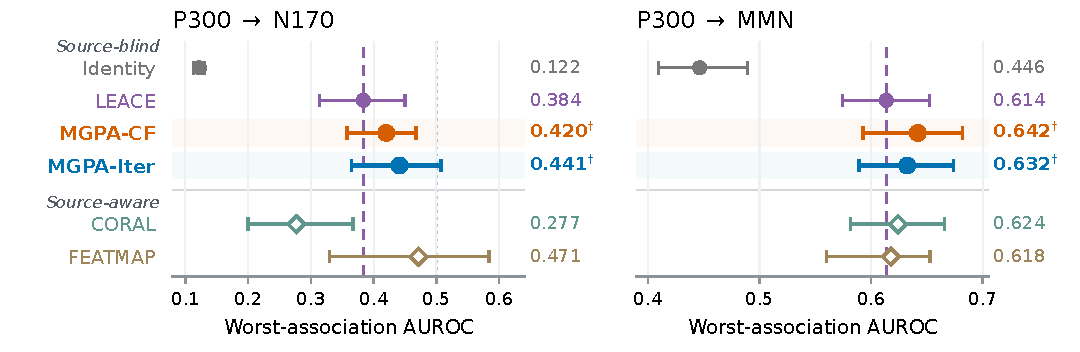
\includegraphics[width=\linewidth]{assets/reuse_worst_preview.pdf}
\caption{\textbf{Reusing a P300-selected correction.}
Absolute worst-association AUROC of frozen N170/MMN shortcut-trained heads;
whiskers show marginal 95\% participant-bootstrap intervals.
Dashed: LEACE; dotted: chance; hollow: source-aware methods.
$\dagger$: paired 95\% interval for the gain over LEACE entirely above zero.
Intervals condition on fitted maps and are unadjusted for multiplicity;
panel ranges differ.}
\label{fig:reuse}
\end{figure}

Both MGPA constructions improve worst-association AUROC over LEACE on
the two transfer tasks (Table~\ref{tab:reuse-main}). Iterative MGPA gains
$.0574$ $[.0338,.0831]$ on N170 and $.0188$ $[.0040,.0241]$ on MMN;
Closed-form MGPA gains $.0364$ $[.0049,.0667]$ and $.0282$ $[.0021,.0343]$,
respectively. Control-head AUROC stays close to identity across all three
tasks. FEATMAP has the highest N170 worst-association score, with lower
N170 and MMN control-head scores; the grouped comparison retains its
source-aware deployment interface.

Figure~\ref{fig:reuse} compares absolute worst-association performance on
both transfer tasks, with LEACE as a reference.
Together, the experiments connect selective correction of representations
to reusable changes in downstream prediction.
